\documentclass{article}
\usepackage[T1]{fontenc}
\usepackage[utf8]{inputenc}
\usepackage[margin=1in]{geometry}
\usepackage{fancyhdr} 
\usepackage{listings}
\lstdefinelanguage{JavaScript}{
  keywords={break, case, catch, continue, debugger, default, delete, do, else, finally, for, function, if, in, instanceof, new, return, switch, this, throw, try, typeof, var, void, while, with},
  keywordstyle=\color{blue}\bfseries,
  ndkeywords={class, export, boolean, throw, implements, import, this},
  ndkeywordstyle=\color{darkgray}\bfseries,
  identifierstyle=\color{black},
  sensitive=false,
  comment=[l]{//},
  morecomment=[s]{/*}{*/},
  commentstyle=\color{purple}\ttfamily,
  stringstyle=\color{red}\ttfamily,
  morestring=[b]',
  morestring=[b]"
}
\lstdefinelanguage{Python3}{
  keywords={False, class, finally, is, return, None, continue, for, lambda, try, True, def, from, nonlocal, while, and, del, global, not, with, as, elif, if, or, yield, assert, else, import, pass, break, except, in, raise},
  keywordstyle=\color{blue}\bfseries,
  ndkeywords={self},
  ndkeywordstyle=\color{darkgray}\bfseries,
  identifierstyle=\color{black},
  sensitive=true,
  comment=[l]{\#},
  morecomment=[s]{"""}{"""},
  commentstyle=\color{purple}\ttfamily,
  stringstyle=\color{red}\ttfamily,
  morestring=[b]',
  morestring=[b]"
}
\usepackage[ruled,vlined]{algorithm2e}
\usepackage{amsthm}
\usepackage{amsfonts}
\usepackage{amssymb}
\usepackage{graphicx}
\usepackage[dvipsnames]{xcolor}
\usepackage{xy}
% \usepackage{url} % Commented out because hyperref provides similar functionality
\usepackage{parskip}
\usepackage{comment}
\usepackage{setspace}
\usepackage{enumerate}
\usepackage{multirow}
\usepackage{hyperref}
\usepackage{caption}
\usepackage{subcaption}
\usepackage{booktabs}
\usepackage{wrapfig}
\usepackage{times}
\usepackage{listings}

\captionsetup[figure]{font={small,it}}

\usepackage[backend=biber,style=numeric,sortcites,maxbibnames=99]{biblatex}
\addbibresource{references.bib}

\newcommand{\HRule}{\rule{\linewidth}{0.5mm}}
\newcommand{\Hrule}{\rule{\linewidth}{0.3mm}}
\newcommand{\classnum}{CS-GY 6313 B}

\makeatletter% since there's an at-sign (@) in the command name
\renewcommand{\@maketitle}{%
  \parindent=0pt% don't indent paragraphs in the title block
  \centering
  {\Large \bfseries\textsc{\@title}}
  \HRule\par%
  \textit{\@author \hfill \classnum}
  \par
}
\makeatother% resets the meaning of the at-sign (@)

\title{Assignment 3: Interactive Visualization} 
\author{Ivan Aristy — iae225}
% \classnum

\begin{document}
  \maketitle % prints the title block
  \thispagestyle{empty}
  % \vspace{-15pt}

\section{Interactive Visualization}
\label{sec:sec1}

\subsection{Question }
\label{subsec:subsec1}

\textbf{How has my champion's win rate changed over time? Is my champion still strong in the current meta?}

I want the user to easily see the win rate of their champion over time. 
Winrate is a key metric in League of Legends, as it is a good indicator of how strong a champion is in the current meta.
This would allow the user to see how their champion has been impacted in recent patches.

Winrate is not a direct representation of power, since some champions are harder to play than others.
Easy champions usually have high winrates, while hard champions have lower winrates.
Additionally, hyper-specific champions have really high winrates, since they are only played in specific situations.

Nevertheless, patterns in winrates can be indicative of power. For example, a 2\% growth in winrates
over a patch can be indicative of a very strong relating buff, while a 2\% decrease can be indicative of a strong relative nerf.
Additionally, a winrate that is consistently above 50\% can show that a champion has and is strong in the current meta.

\subsection{Data}
\label{subsec:subsec2}

\subsubsection{Data Source}
\label{subsubsec:Data Source}

Riot's Developer API is very hard to use. In my opinion, it is not well documented, and it is very hard to get the data you want.
Hence, I wll scrape some data off the internet to get the winrate of a champion over time.

Particularly I need:
\begin{enumerate}
  \item The winrate of a champions over time.
  \item The tier of the champion over time.
  \item Visual Assets of the champion.
\end{enumerate}

\subsubsection{Data Retreival} 
\label{subsubsec:Data Retreival}

To get winrate data, I will scrape \url{https://lolalytics.com/lol/tierlist/} for the winrate and tier of a champion over time.

After analyzing the beautiful soup output, the relevant information for a champion 
is contained in a div with the class \texttt{flex justify-around border border-[\#333333] p-2 text-center}.
For the next div, we will skip the explanation, but it uses a similar process to the code below.

\begin{figure}[ht] % Change the position of your figure https://www.overleaf.com/learn/latex/Positioning_images_and_tables
  \centering
  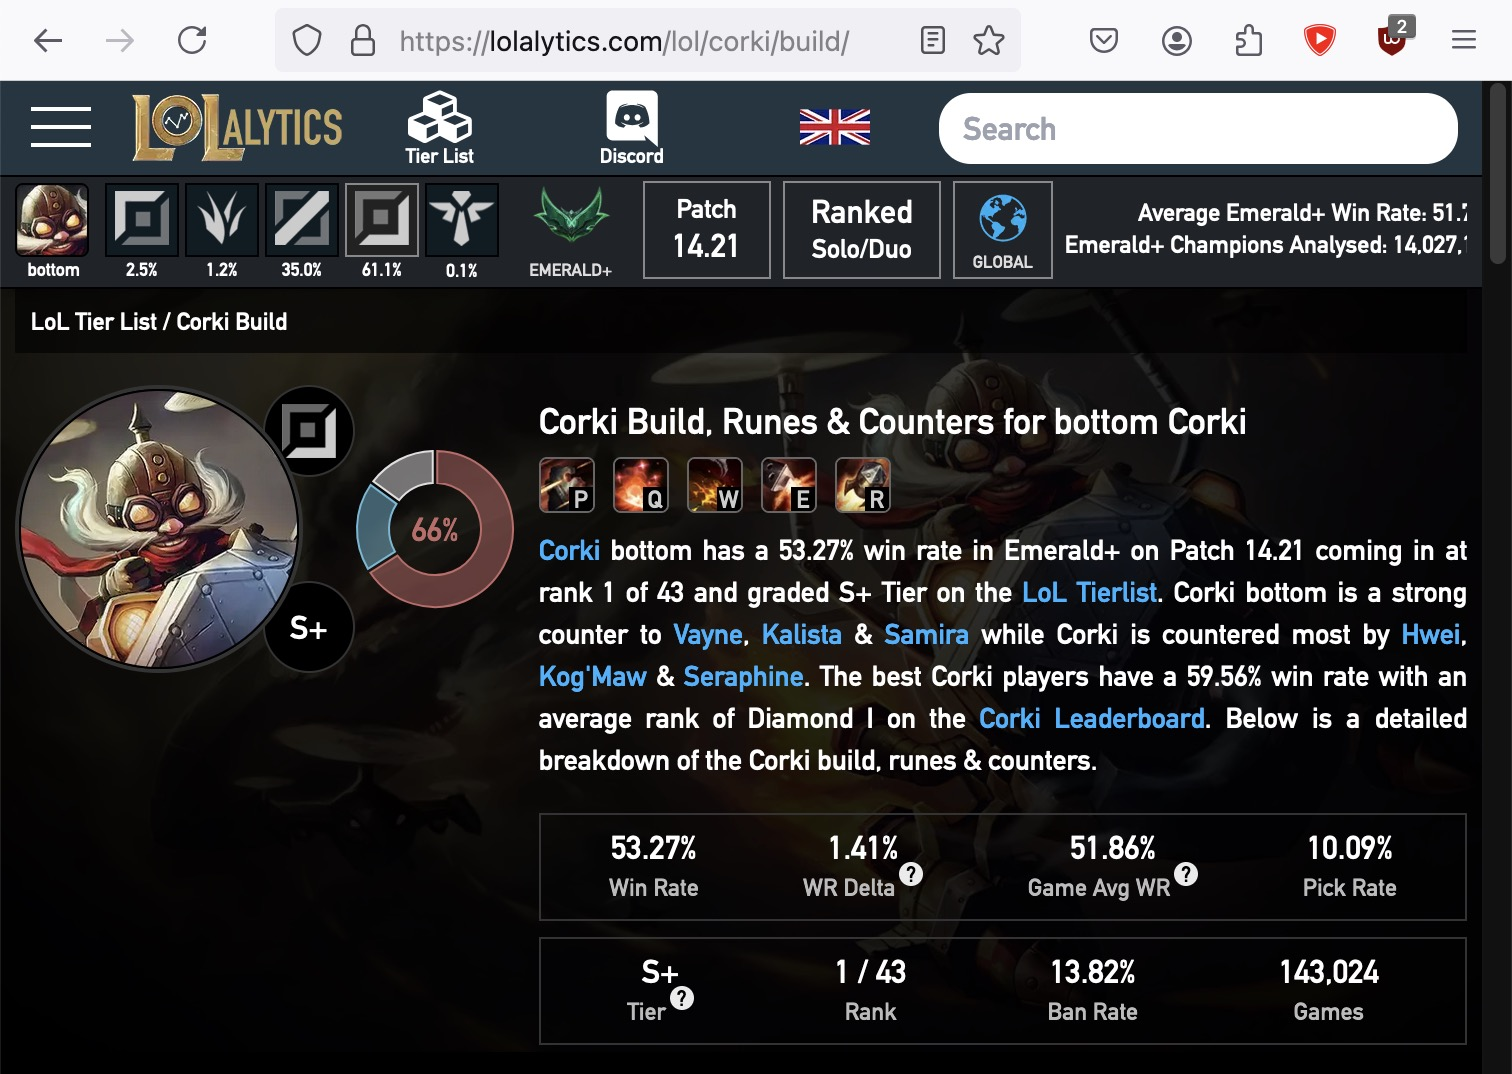
\includegraphics[width=0.75\textwidth]{figs/website.jpg}
  \caption{
      Corki's champion page.
  }
  \label{fig:fig1}
\end{figure}

\begin{lstlisting}[language=Javascript]
  container_div = soup.find('div', class_='flex justify-around 
  border border-[#333333] p-2 text-center')
  if container_div:
      # Find all the individual sections within this container
      sections = container_div.find_all('div', recursive=False)
      
      for section in sections:
          value_div = section.find('div', class_='mb-1 font-bold')
          if value_div:
              value = value_div.get_text(strip=True)
              row_1_data.append(value)
  print(row_1_data)
\end{lstlisting}

In \autoref{fig:fig1} the relevant data would be the eight values from "Win Rate"
to "Games". However, this information is only for one patch, so the backend
function will also receive a parameter to indicate the patch to scrape.

\subsubsection{Serving Backend Server} 
\label{subsubsec:Serving Backend Server}

We are using FastAPI to expose the data to the frontend. 
To accurately model the data, I created the following interface:

\begin{lstlisting}[language=Python3]
class ChampionInstance(BaseModel):
  name: str
  patch: float
  win_rate: float
  win_rate_delta: float
  modified_winrate: float
  pick_rate: float
  tier: str
  rank: int
  ban_rate: float
  games: int
\end{lstlisting}

and exposed the following function to the frontend:

\begin{lstlisting}[language=Python3]
@app.get("/test/{champion_name}&{patch_version}")
async def test(champion_name: str, patch_version: str):
  testChampion: ChampionInstance = 
    await api.get_champion_data(champion_name, patch_version)
  return testChampion
\end{lstlisting}

All the functions used were asynchronous, since load times were a complaint 
I received from my peers while showing them the assignment.

% \begin{figure}[ht] % Change the position of your figure https://www.overleaf.com/learn/latex/Positioning_images_and_tables
%   \centering
%   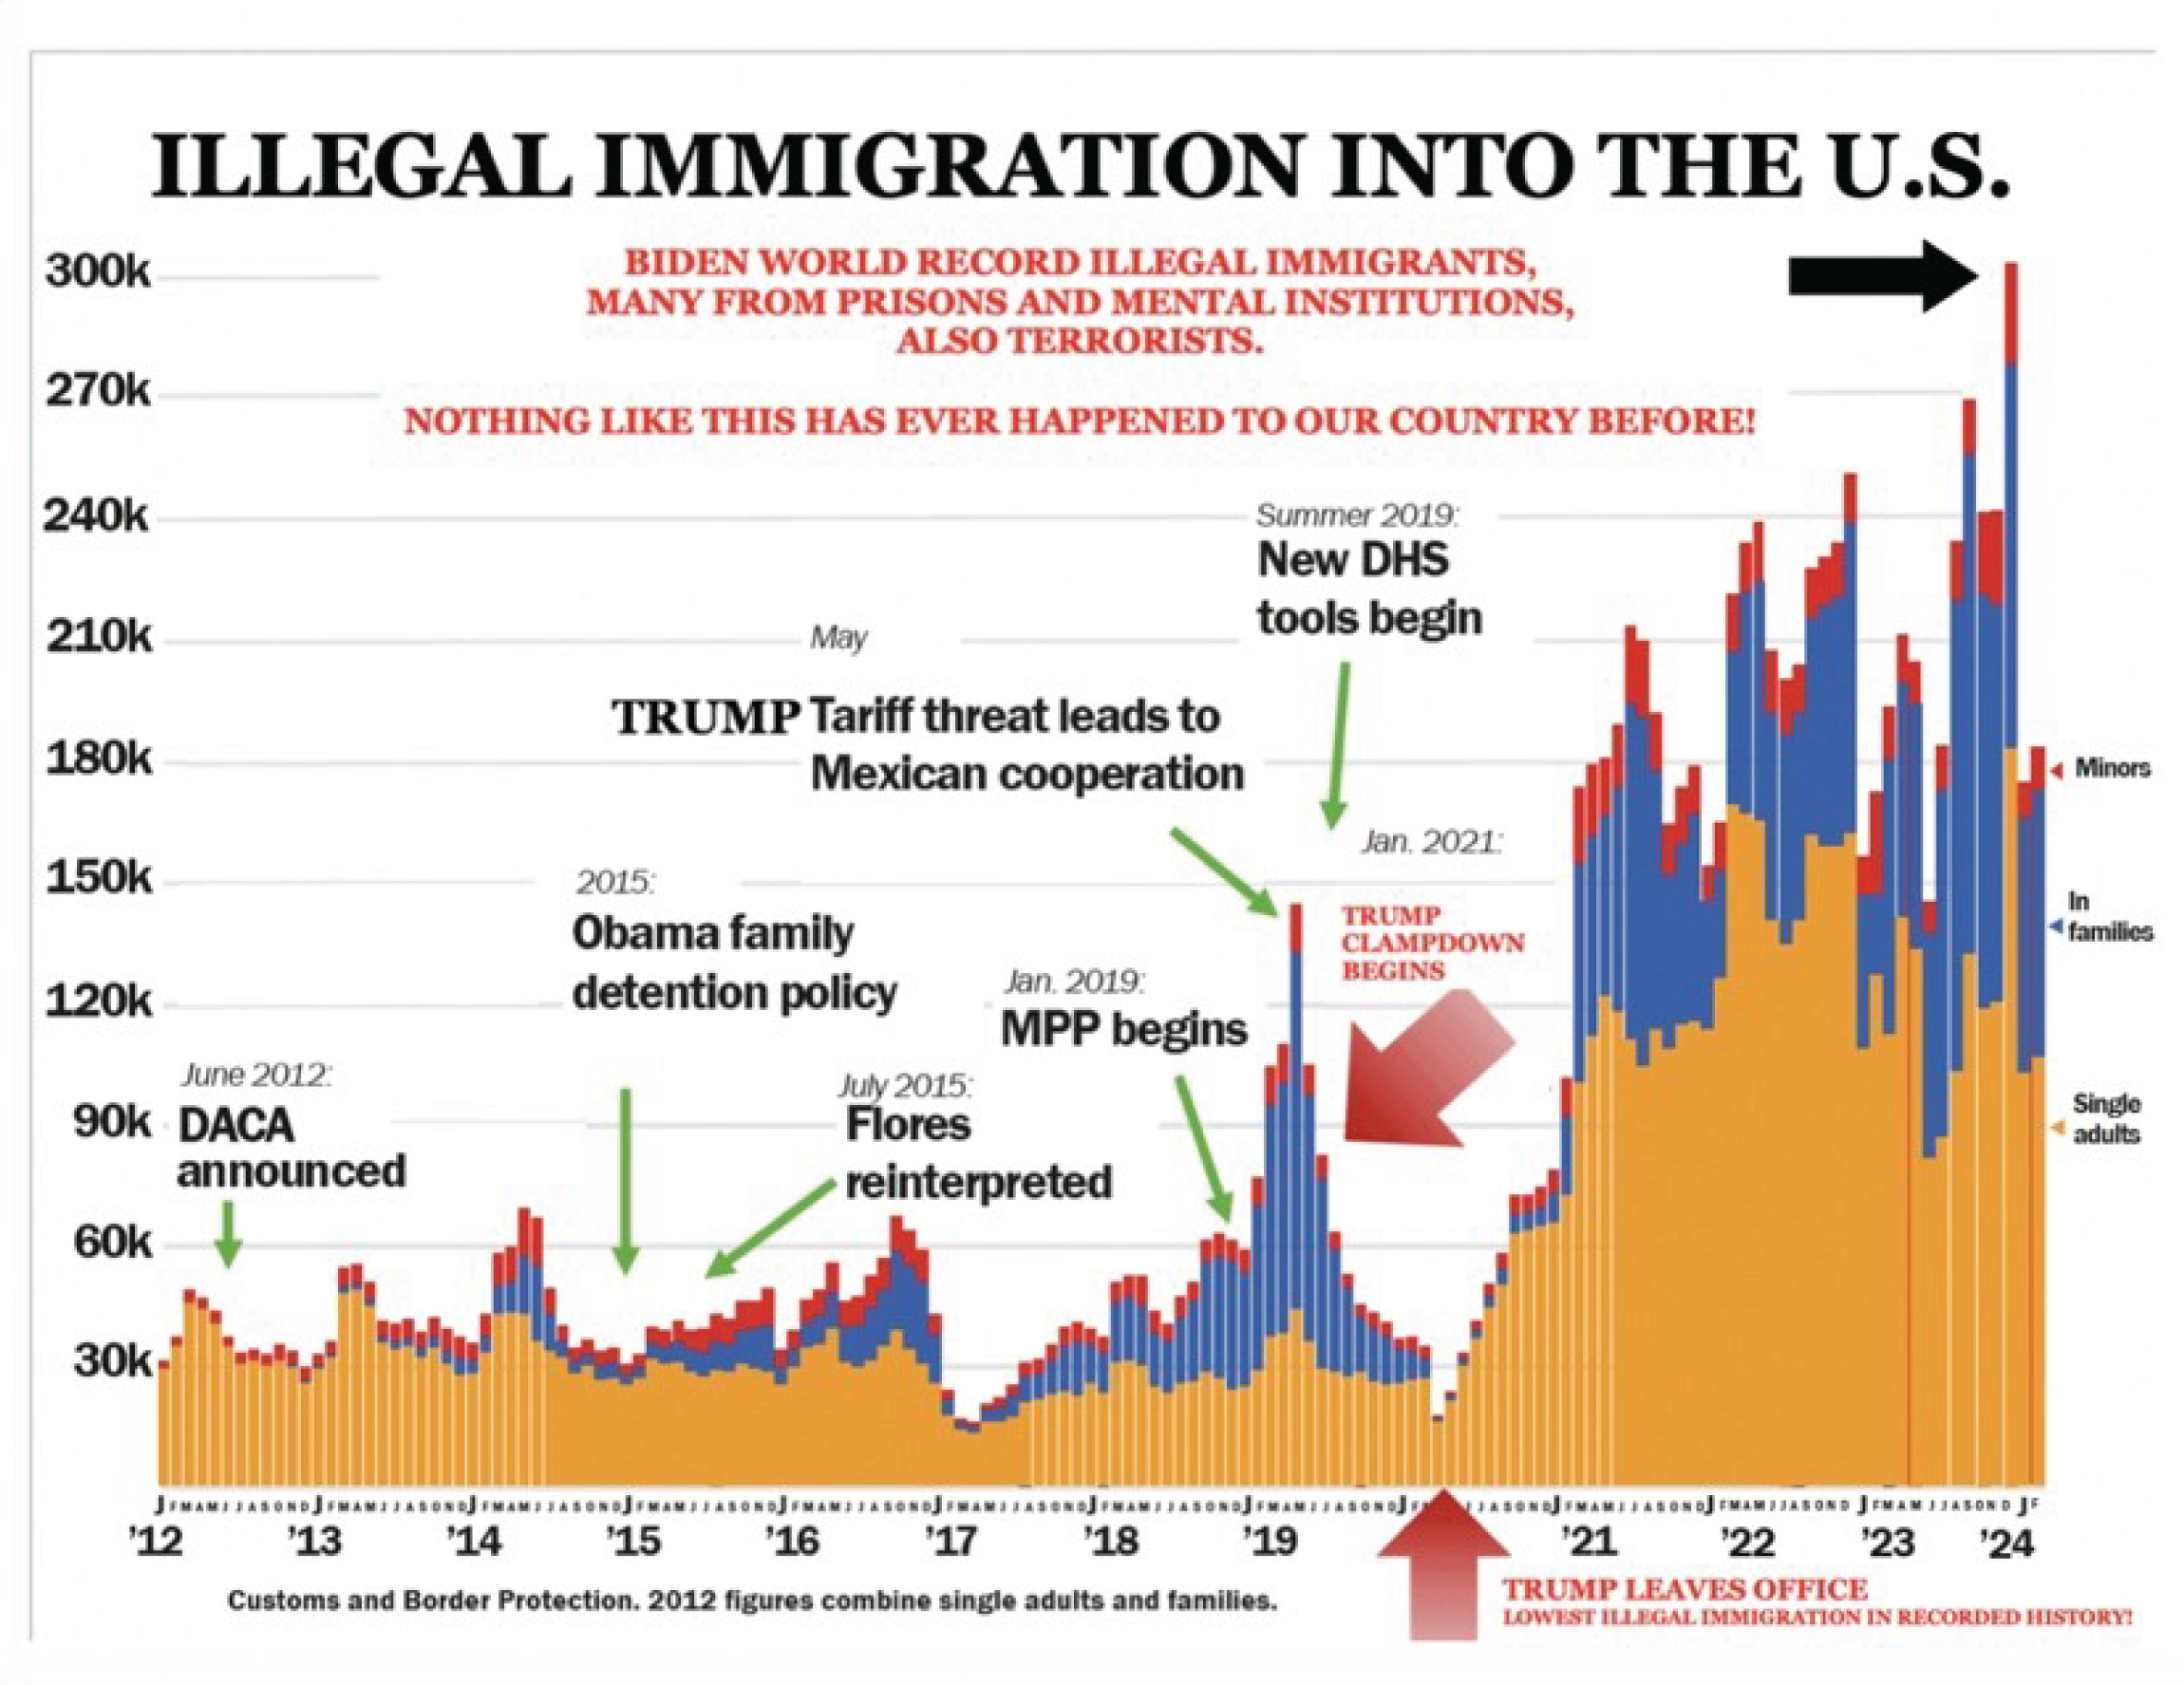
\includegraphics[width=0.75\textwidth]{figs/Trump Chart.png}
%   \caption{
%       Trump's Illegal Immigration Chart
%   }
%   \label{fig:fig1}
% \end{figure}




\begin{refcontext}[sorting=nyt]
\printbibliography
\end{refcontext}

\end{document}

